\documentclass{article}
\usepackage[latin1]{inputenc}
\usepackage[spanish]{babel}
\usepackage{amsmath, amsthm, amsfonts}
\usepackage{cite}
\usepackage{listings}
\usepackage{color}
\usepackage{graphicx}
\usepackage{enumitem}

\definecolor{dkgreen}{rgb}{0,0.6,0}
\definecolor{gray}{rgb}{0.5,0.5,0.5}
\definecolor{mauve}{rgb}{0.58,0,0.82}

\lstset{frame=tb,
  language=Python,
  aboveskip=3mm,
  belowskip=3mm,
  showstringspaces=false,
  columns=flexible,
  basicstyle={\small\ttfamily},
  numbers=none,
  numberstyle=\tiny\color{gray},
  keywordstyle=\color{blue},
  commentstyle=\color{dkgreen},
  stringstyle=\color{mauve},
  breaklines=true,
  breakatwhitespace=true,
  tabsize=3
}


\title{Optimizaci�n de Flujo en Redes:\\
		Reporte 2}
\author{Alcantar G�mez Alan Arnoldo\\
  \small{Matricula: 1935040}
}

\begin{document}
\maketitle

\section{Introducci�n}

El presente trabajo se desarroll� para introducir las herramientas de programaci�n \textbf{Python}: \textit{Clases} y \textit{funciones}, con el objetivo de reestructurar el c�digo empleado en el reporte 1 y tener un c�digo m�s robusto y flexible.  


\section{Descripci�n del sistema termodin�mico}
Consid�rese un conjunto de N part�culas ubicadas de forma aleatoria que est�n sometidas a un campo de temperatura uniforme a lo largo del eje \textit{x}, y disminuye a lo largo del eje \textit{y}, de este modo la temperatura de cada part�cula estar� dada por su posici�n. Por �ltimo, definir que todo el sistema se encuentra en un espacio cuadrado de 1 metro.\\


El radio de interacci�n de la part�cula $i$ se modela como la multiplicaci�n entre su coordenada $y(i)$ y un par�metro $\alpha$. Por otro lado la temperatura de la part�cula $i$, $T(i)$, se modela como la multiplicaci�n entre su coordenada $y(i)$ y la temperatura m�xima del sistema $T_{max}$.

\begin{equation}\label{eq:radio}
  R(i) = y(i)*\alpha
\end{equation}

\begin{equation}\label{eq:temp}
  T(i) = y(i)*T_{max}
\end{equation}

De modo que la part�cula $i$ podr� interaccionar con cualquier particula \textit{j} ($i \neq j$) si la distancia entre estas es igual o menor al radio de interacci�n de la part�cula $i$.

\begin{equation}\label{eq:cond}
  D(i,j) \leq R(i)
\end{equation}

\section{Descripci�n del algoritmo para representar el sistema por medio de un grafo}
Los par�metros necesarios para generar el grafo son n (n�mero de part�culas), t (temperatura m�xima), a (par�metro $\alpha$) y modo (simple, dirigido, ponderado, campechano).\\

Los componentes principales del c�digo son: una \textit{clase} llamada Grafo y dentro de ella existen tres \textit{funciones}.

\begin{itemize}
	\item \textit{vertices(self,n,t)}: generar n nodos, cuyas coordenadas y temperaturas son guardadas 
	\item \textit{unir(self,n,a)}: genera la arista entre los nodos $i, j$ si y solo si cumple con la condici�n \ref{eq:cond}
	\item \textit{graficar(self,modo)}: genera el archivo de salida para \textbf{Gnuplot} de acuerdo al tipo de grafo que se desea
\end{itemize}



\begin{lstlisting}
from math import sqrt
from random import random
class Grafo:

    def __init__(self):
        self.nodos = dict()     
        self.aristas = dict()   
        self.vecinos = dict()   

    def vertices(self, i, t):
    	for j in range(i):
    		y = random()
    		self.nodos[j] = (random(), y, y*t)
    		
    def unir(self, i, alpha):
	    for k in range(i-1):
	    	for l in range(k+1, i):
	    		d = sqrt((self.nodos[l][0] - self.nodos[k][0])**2 + (self.nodos[l][1] - self.nodos[k][1])**2)
	    		if d <= self.nodos[k][1]*alpha:
	    			xm = (self.nodos[l][0] + self.nodos[k][0])/2 
	    			ym = (self.nodos[l][1] + self.nodos[k][1])/2
	    			w = (self.nodos[l][2] + self.nodos[k][2])/10
	    			self.aristas[(k,l)] = (xm, ym, w)
	    			if not k in self.vecinos:
	    				self.vecinos[k] = set()
	    			if not l in self.vecinos:
	    				self.vecinos[l] = set()
	    			self.vecinos[k].add(l)
	    			self.vecinos[l].add(k)
    		
\end{lstlisting}

\section{Resultados}
A continuaci�n, se presentan los resultados.

\begin{figure}[h]
\label{tab:regiones}

\centering
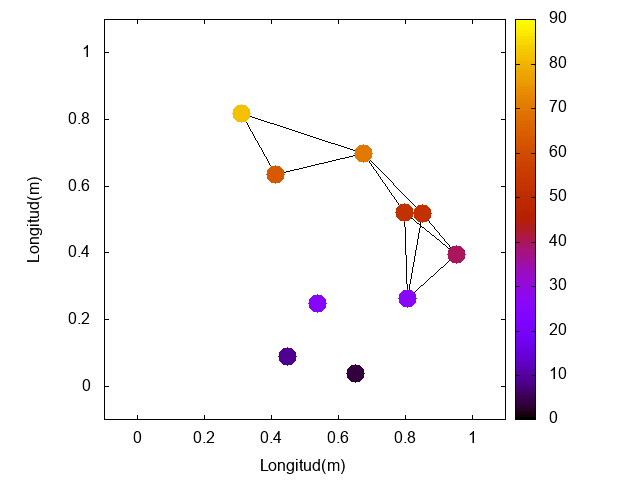
\includegraphics[width = 0.9\textwidth]{simple.png}

\caption{Gr\'afica de interacciones, $N=10$, $T_{max}=100$ y $\alpha=0.7$, $modo:simple$.}
\end{figure}

\pagebreak

\begin{figure}[h]
\label{tab:interacciones}

\centering
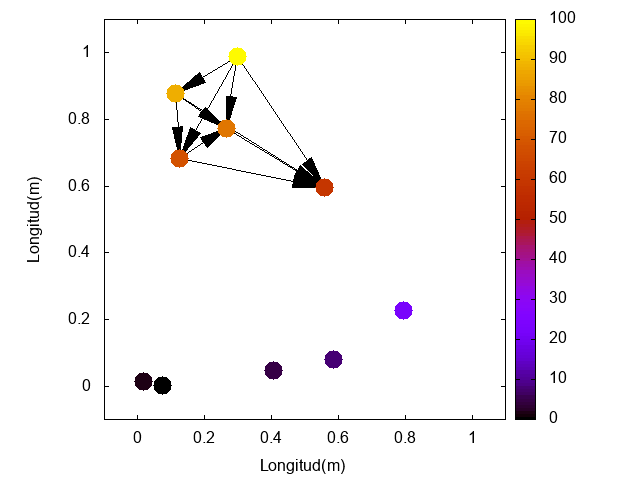
\includegraphics[width = 0.9\textwidth]{dirigido.png}

\caption{Gr\'afica de interacciones, $N=10$, $T_{max}=100$ y $\alpha=0.7$, $modo:dirigido$.}
\end{figure}

\pagebreak

\begin{figure}[h]
\label{tab:interacciones}

\centering
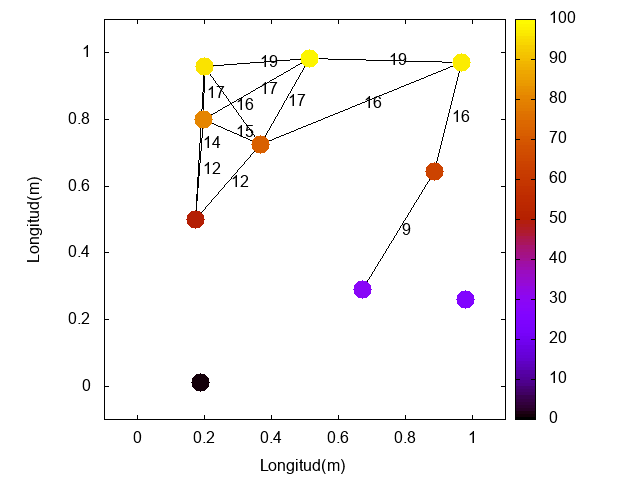
\includegraphics[width = 0.9\textwidth]{ponderado.png}

\caption{Gr\'afica de interacciones, $N=10$, $T_{max}=100$ y $\alpha=0.7$, $modo:ponderado$.}
\end{figure}

\pagebreak

\begin{figure}[h]
\label{tab:interacciones}

\centering
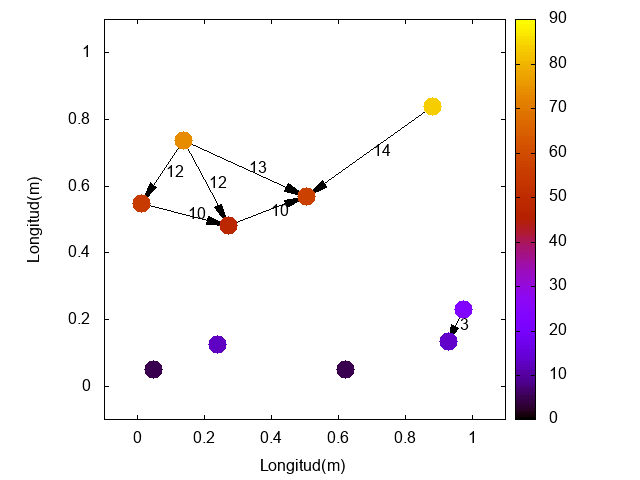
\includegraphics[width = 0.9\textwidth]{campechano.png}

\caption{Gr\'afica de interacciones, $N=10$, $T_{max}=100$ y $\alpha=0.7$, $modo:campechano$.}
\end{figure}

\pagebreak

\section{Conclusi�n}

Como se observ� en la parte de experimentaci�n el utilizar \textit{clases} y \textit{funciones} permite que podamos generar varios tipos de grafos a trav�s de los par�metros con los que trabajen cada una de las \textit{funciones}. Esto nos permite utilizar el mismo c�digo para resolver distintos problemas donde las direcciones o capacidades entre los nodos tengas una caracter�stica importante.



\end{document}